\documentclass{article}
\usepackage{amsthm}
\usepackage[utf8]{inputenc}
\usepackage{graphicx}
\begin{document}
Nathan Helms: CMSC208: HW2
\begin{enumerate}
\item
Use the Pumping Lemma to show that the language is not regular
$$\{www | w \in \{a,b\}^\ast\}$$
\newline
To prove that the language above is not regular with the pumping lemma, it must first be broken down properly.
\newline
\newline
$$w = \{a,b\}^\ast$$
$$s = xy^nz$$
Example for why the language is not regular by following the formula of s
\newline
\begin{center}
$x = aaabb$ $y^n = aabbab$ $z = ababab$
\end{center}
$$y^n = aaab^\ast? $$
$$y^n = aabba^\ast? $$
Both of the above substitutions for $y^n$ would not properly conform to the pumping lemma, therefore the language is not regular
\item
Construct a DFA to recognize the language $\{w | w $ is any string except $11$ or $111\}$
\newline
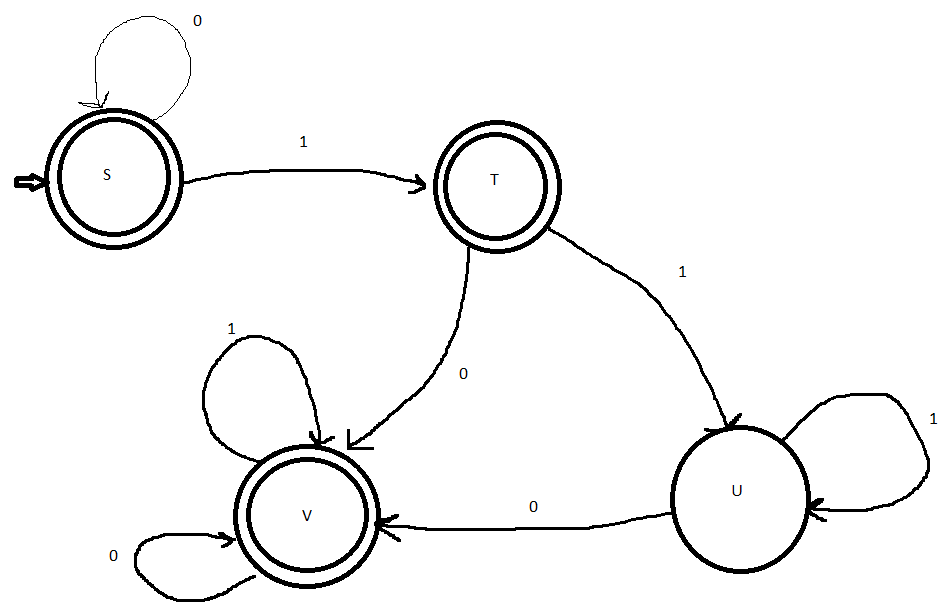
\includegraphics[scale=0.5, height=7cm]{DFA}
\newline
\item
Give a context-free grammars that generates the following languages:
\newline
\begin{center}
a) $\{w | w$ contains at least three $1$s$\}$
b) $\{w | w$ has an odd length$\}$
\end{center}
a) $$W \Rightarrow W + T | T$$
$$T \Rightarrow W | 1$$
b) $$W \Rightarrow W + T | T$$
$$T \Rightarrow ??? $$
\newline
\newline
\item
Give informal descriptions for pushdown automata for the previous problem's languages
\newline
\newline
For letter a, have a check state for if a 1 is passed, so that it pushes it on the stack. When popping, have several states for pushing at least 3 singular 1s throughout the stack. if the end character is reached prior to 3 singular 1s being popped, have the PDA reject. If three 1s were popped, and then the end character is reached, accept.
\newline
\newline
For letter b, Have two end states when popping the stack. One accepting the special character, and one accepting either a 0 or a 1. If the special character is recognized, reject, as if there was an odd number of pushes/pops, there would be a 0 or 1 left in the stack, in which the PDA would accept if that was the case.
\item
Using the following context-free grammar, give a parse tree for the strings
\newline
a) a+a+a
\newline
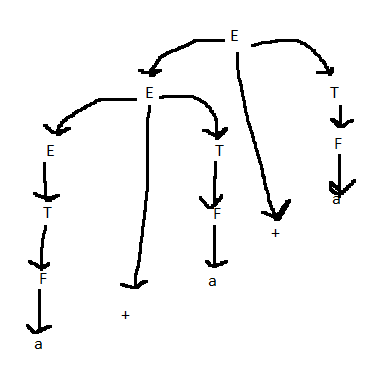
\includegraphics[scale=0.75]{CFG1}
\newline
b) ((a))
\newline
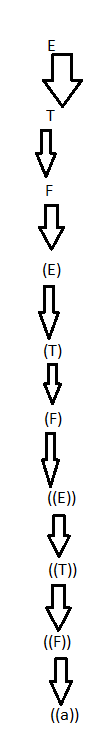
\includegraphics[scale=0.75]{CFG2}
\end{enumerate}
\end{document}
